\section{Descripción y caracterización detallada del problema}

\subsection{Criterios de selección del problema}

De los tres problemas identificados en la Introducción, se seleccionó el desabastecimiento de medicamentos y falta de alternativas usando los siguientes criterios:

\begin{enumerate}
	\item \textbf{Impacto social medible:} Afecta directamente a pacientes con enfermedades crónicas. En 2024 se registraron más de 150,000 tutelas relacionadas con falta de acceso a medicamentos.
	
	\item \textbf{Urgencia temporal:} Crisis activa que requiere soluciones inmediatas.
	
	\item \textbf{Viabilidad técnica con IA:} Puede abordarse con CNN y KNN existentes.
	
	\item \textbf{Disponibilidad de datos:} Existen fuentes públicas (INVIMA, MinSalud).
	
	\item \textbf{Factibilidad de implementación:} Solución de software más rápida que cambios estructurales.
	
	\item \textbf{Empoderamiento del usuario:} Pone información directamente en manos de pacientes.
	
	\item \textbf{Escalabilidad:} Puede expandirse fácilmente a más medicamentos y usuarios.
\end{enumerate}

\subsection{Caracterización detallada del problema seleccionado}

La Universidad Javeriana en un estudio, comenta que el asunto no reside en la ausencia física de los medicamentos, sino que, tal y como mencionaba el Universal, es en todo el abastecimiento, precisamente por toda la crisis financiera que vienen arrastrando \cite{diaz2025}.

La falta de abastecimiento y entrega de medicamentos no solo afecta a los pacientes sino también a hospitales. Durante el año pasado, por suspensión de actividades de empresas que se encargaban de la producción de medicamentos a nivel nacional, el Ministerio de Salud emitió que llegó a haber una escasez de fármacos vitales, tales como la norepinefrina o la vasopresina (usados en UCI principalmente). A saber: En el caso de la norepinefrina, el mercado está cubierto en un 26\% por Laboratorios Ryan, que dispone de 120.000 ampollas mensuales entre septiembre y diciembre. Sin embargo, esta cantidad no ha sido suficiente para cubrir la demanda, motivo por el cual el medicamento permanece en la lista de vital no disponible desde 2018.

Debido a esto, se tuvieron que otorgar licencias y autorizaciones de importación a empresas externas para un correcto abastecimiento, en donde gracias a las empresas como Holland Group, Pisa Farmacéutica, Reprefarco y Sicmafarma, pudieron llegar de la mano de Reprefarco unas 100.000 unidades, además de la empresa Nextpharmasourcing que otorgó 3.700 cajas de 10 ampollas cada una, dando un gasto más a todo el que se viene arrastrando \cite{saavedra2025}.

Asimismo, a pesar de que se viene incrementando el desembolso por parte de los colombianos en la compra de medicamentos, dando un crecimiento en el gasto privado, no garantiza una traducción en acceso oportuno a estos medicamentos, en donde se presentan demoras extensas, además de una falta de disponibilidad y un alza en los precios, generando una presente y creciente sensación de inconformismo entre la sociedad dependientes de los medicamentos (enfermedades crónicas, patologías huérfanas o tratamientos de alto costo como el cáncer) \cite{calero2025}.

% PRIMERA IMAGEN - Tabla de categorías del gasto
\begin{figure}[H]
	\centering
	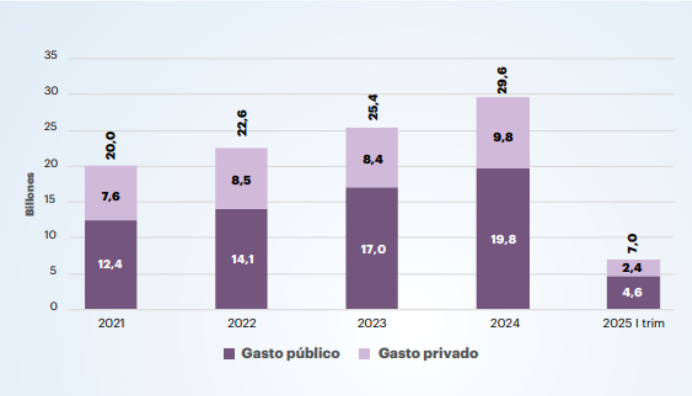
\includegraphics[width=0.90\textwidth]{img/gasto.png}
	\caption{Detalle del gasto en salud por categorías 2021-2025}
	\label{fig:gasto}
\end{figure}

% SEGUNDA IMAGEN - Gráfica de evolución
\begin{figure}[H]
	\centering
	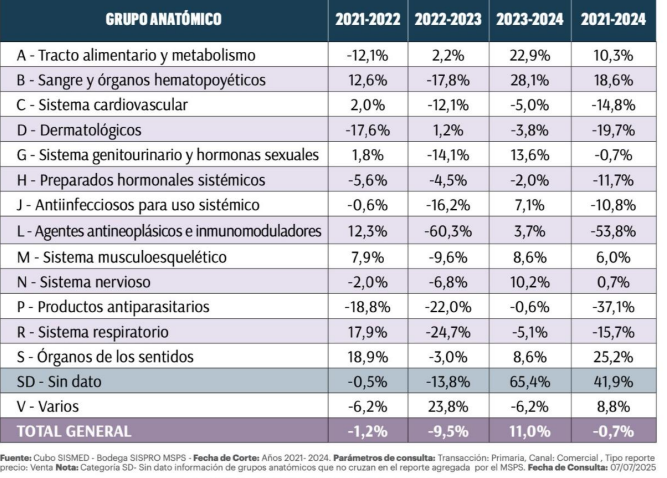
\includegraphics[width=0.85\textwidth]{img/evolucionGasto.png}
	\caption{Evolución del gasto privado en medicamentos en Colombia 2021-2025}
	\label{fig:evolucion}
\end{figure}

Como se puede evidenciar en las gráficas anteriores, el gasto privado en salud se fue en alza en los últimos años, pasando de ser de 20 billones a 29.2 billones entre 2021 y 2024, además de un aumento nominal del 48.0\% y del 13.8\% después de inflación.

Igualmente es válido mencionar que el gasto en medicamentos no incluye los costos adicionales asociados a la gestión para la disposición de las medicinas en los gestores farmacéuticos o prestadores de servicios de salud \cite{acemi2025}.

Como bien se mencionó previamente, no es un tema sencillo de encontrarle y/o darle una solución exacta, para la magnitud que representa ante una sociedad donde existe un grupo de personas que dependen de medicamentos para su día a día debido a distintas complicaciones. Del mismo modo, al ser una situación país grande, se genera la falsa esperanza que será el gobierno que logre solucionar todo en tiempo récord y la sociedad se quedará esperando hasta que exista una garantía, pero esa espera solo genera una cadena dominó de más problemas, en vez de poder darle alternativas y soluciones temporales utilizando la tecnología como medio para ello.

\pagebreak